%!TEX root = dolgozat.tex
%%%%%%%%%%%%%%%%%%%%%%%%%%%%%%%%%%%%%%%%%%%%%%%%%%%%%%%%%%%%%%%%%%%%%%%
\chapter{Neurális hálózatok}\label{ch:INTRO}
%%%%%%%%%%%%%%%%%%%%%%%%%%%%%%%%%%%%%%%%%%%%%%%%%%%%%%%%%%%%%%%%%%%%%%%

\begin{osszefoglal}
Ebben a fejezetben megnézzük a biológiai modellt aminek a mintájára a mesterséges neuronokat létrehozták, megismerkedünk a mesterséges neuronokkal és a neurális hálókkal majd pedig megnézzük hogyan is tanulnak ezek.
\end{osszefoglal}

\section{Bevezető}
\subsection{Biológiai modell}

Az idegsejtek (neuronok) az idegrendszer alkotóelemei. A neuron jeleket fogad és ezekre megfelelő választ generál. Az emberi idegrendszer nagyon komplex műveletek elvégzésére képes rövid idő alatt. Mivel ennek analógjára hozták létre a mesterséges neurális hálókat, ezért fontos a biológiai alapok megismerése.

A \ref{fig:idegsejt} ábrán látható egy idegsejt és annak részei. A dendritek más neuronokkal állnak kapcsolatban és a bejövő információt szállítják. A beérkezett információ feldolgozását a sejtmag hajtja végre. Az idegrost egy szigetelt vezető aminek az a feladata, hogy továbbszállítsa az információt. Az axonvégek más neuronok dendritjeivel vannak kapcsolatban, a választ szállítják tovább a velük kapcsolatban levő idegsejteknek. 


\begin{figure}[h]
\centering

\includegraphics[scale=0.5]{images/idegsejt}
\caption{Idegsejt}
\small forrás:\url{http://www.clker.com/clipart-neuron.html}


\label{fig:idegsejt}
\end{figure}


\section{Mesterséges neuronok}\label{sec:INTRO:neurons}
A neuronok a neurális hálók építőkövei. 
\subsection{Szigmoid neuron}

A szigmoid neuron 0 és 1 közötti értékeket kap bementi paraméterként és létrehoz egy kimentet ugyanebben az intervallumban.

\begin{figure}[h]
\centering

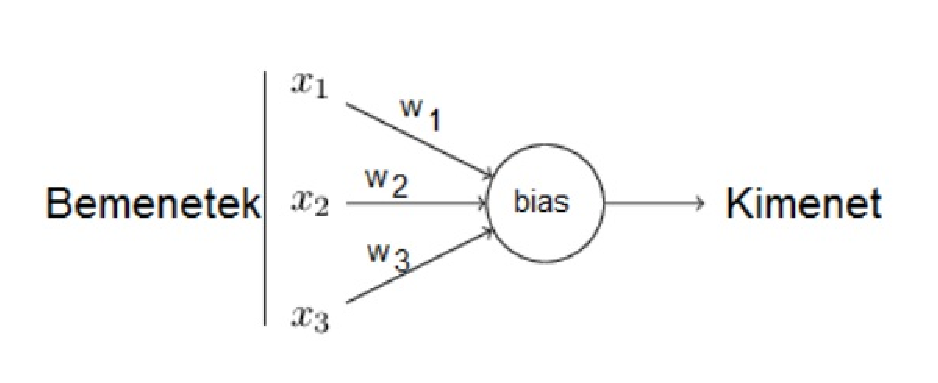
\includegraphics[scale=1]{images/neuron.eps}
\caption{Szigmoid neuron}
\small forrás:\url{http://neuralnetworksanddeeplearning.com/chap1.html}


\label{fig:neuron}
\end{figure}

Mindegyik bemenethez súlyok vannak rendelve, ami azt jelképezi, hogy az illető bemenet mennyire játszik fontos szerepet a neuron kimenetében. Minden neuronhoz tartozik továbbá egy küszöbérték, ami a kisebb rendellenességek javítására szolgál.

A szigmoid neuron kimenete a \ref{eq:1} képlettel számítható ki.

\begin{equation} \label{eq:1}
\sigma(\sum\limits_{i=1}^{n-1} w_{i}x_{i} + b)
\end{equation}

\begin{equation} \label{eq:2}
\sigma(z) = \frac{1}{1+e^{-z}}
\end{equation}

A \ref{eq:2} függvényt aktiválási függvénynek nevezik. Az aktiválási függvény szerepe, hogy a kimenetet egy adott intervallumba szorítsa. Ahogy ez az \ref{fig:sigmoidf} ábrán is látszik, a szigmoid neuron esetében ez az intervallum 0 és 1 között van. 

\begin{figure}[h]
\centering

\includegraphics[scale=0.35]{images/sigmoidf.eps}
\caption{Szigmoid függvény grafikus képe}

\label{fig:sigmoidf}
\end{figure}

A szigmoid neuron egyik tulajdonsága, hogy kis változás a súlyokban kis változást eredményez a kimenetben. Ez egyszerre előny és hátrány is. Előny, mert amikor a kimenet közel van az elvárt kimenethez, a módosítások nem eredményezik azt, hogy a kimenet túlságosan eltávolodjon az elvárttól. Hátrány, mert amikor a kimenet nagyon helytelen, mint például a tanulás elején, hosszú időbe telik a javítása \cite{5}.

\section{Neurális hálók struktúrája}\label{sec:INTRO:architecture}

A neuronokból álló hálózatokat neurális hálóknak nevezzük. A hálózat neuronjai hasonló típusú műveletet végeznek a többi neurontól függetlenül. Egy neuron sok más neuronnal áll kapcsolatban, ahogy ez a biológiai analógiából kikövetkeztethető. Tehát a neurális hálózatok olyan információfeldolgozó eszközök, amelyek párhuzamos, elosztott működésre képesek, lokális feldolgozást végző neuronokból állnak, képesek tanulni, és a megtanult információt felhasználni \cite{10}.

A neuronok egy hálózaton belül általában csak meghatározott számú neuronnal vannak összekötve, és ez a kapcsolat általában egyirányú, ezért a hálózatokat különböző rétegekre szoktuk bontani az összekötések szerint. Az egyes rétegekhez tartozó neuronok az előző réteg neuronjainak kimenetével, vagy a bemenettel, illetve a következő réteg bemenetével vannak összekötve \cite{10}.


\begin{compactenum}
	\item Bemeneti réteg: azok a neuronok találhatók itt, amelyek a bemeneti jel továbbítását végzik a hálózat felé. A legtöbb esetben nem jelöljük őket külön
	\item Rejtett réteg: a tulajdonképpeni feldolgozást végző neuronok tartoznak ide. Egy hálózaton belül több rejtett réteg is lehet
	\item Kimeneti réteg: az itt található neuronok a külvilág felé továbbítják az információt. A feladatuk ugyanaz, mint a rejtett rétegbeli neuronoké \cite{10}.
\end{compactenum}


Ennek függvényében a neuronok elhelyezkedésük alapján három csoportba sorolhatók:
\begin{compactenum}
	\item Bemeneti neuronok
	\item Rejtett neuronok
	\item Kimeneti neuronok
\end{compactenum}


A legtöbb hálózat esetében az egyes rétegek teljesen össze vannak kötve, vagyis egy réteg egy neuronjának kimenete a következő réteg összes bemenetével össze van kötve. A hálózatoknál előforduló számítások elvégzéséhez célszerűbb a hálózatokat különböző mátrixokkal jellemezni. A bemeneteket elegendő egy darab vektorba rendezve ábrázolni, ez N bemenet esetén egy N-es vektort jelent. Az egyes rétegek közötti súlyokat hasonlóan a bemenetekhez mátrixokba szoktuk rendezni. Ez a következőképpen néz ki: ha az l. rétegben n darab neuron van az l+1. rétegben pedig m, akkor a köztük lévő súlyok száma n x m. Ez mátrixba rendezve egy m x n-es mátrixot jelent, amelynek oszlopai az l. réteg neuronjait, sorai az l+1. réteg neuronjait reprezentálják \cite{10}. 

\begin{figure}[h]
\centering

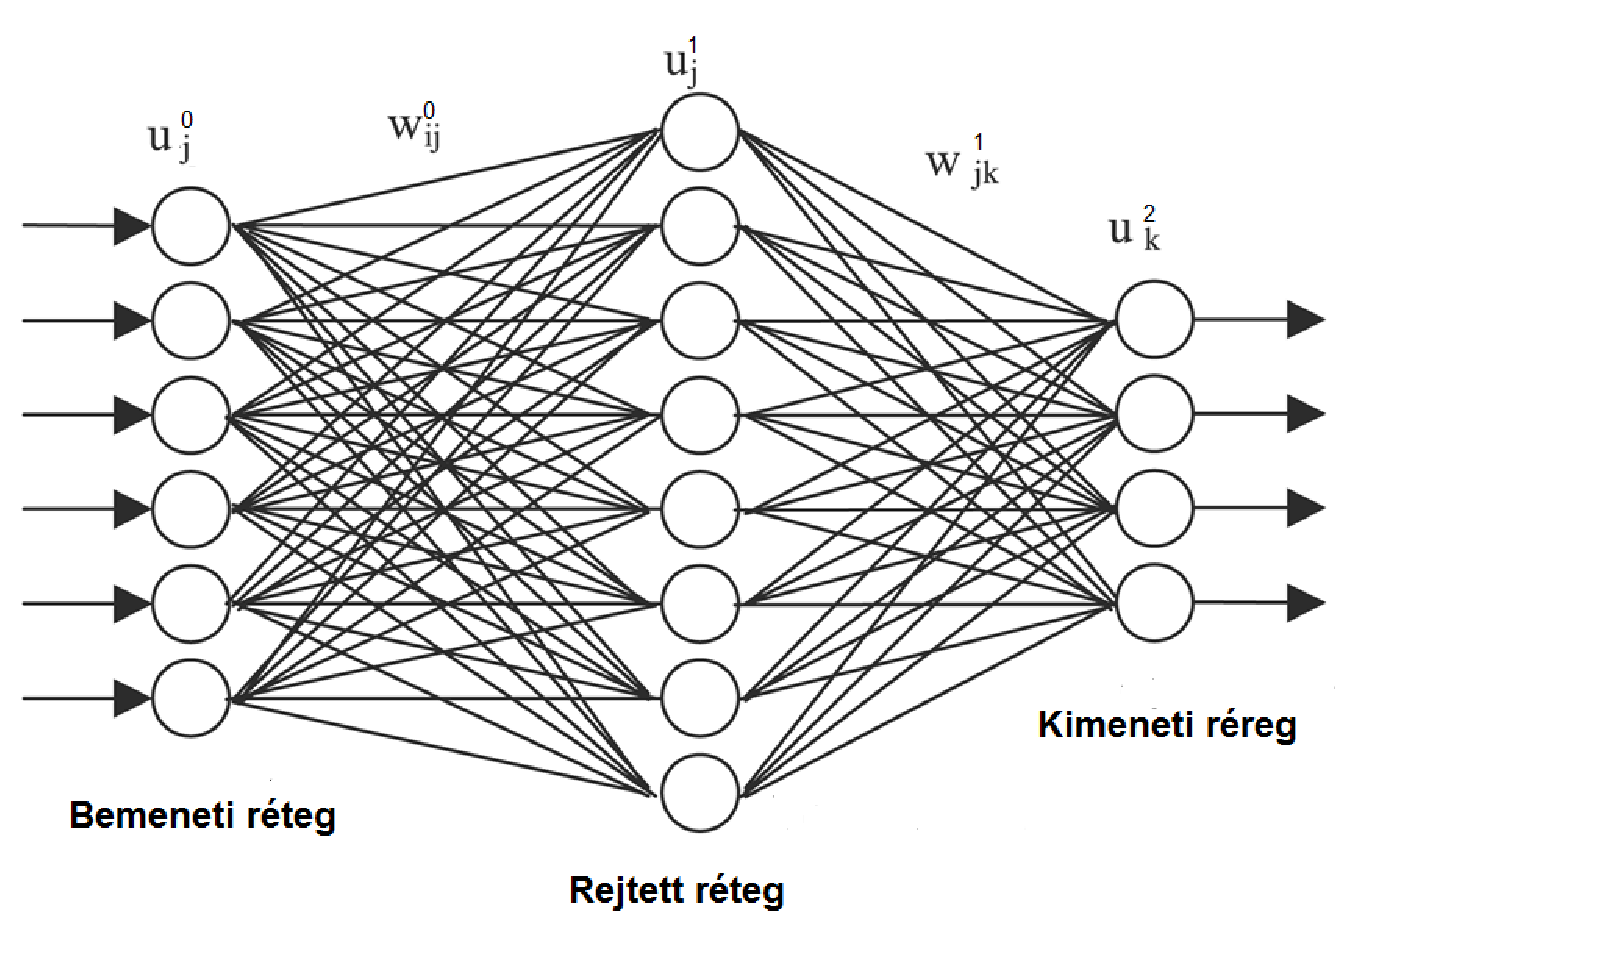
\includegraphics[scale=0.5]{images/net.eps}
\caption{Egyszerű neurális háló}

\label{fig:net}
\end{figure}

A \ref{fig:net} ábrán egy egyszerű szigmoid neuronokból álló neurális háló látható. A súlyvektorok mérete már ennél a kis példánál is viszonylag nagy, ezért egy nagy hálónál ezek az értékek jelentősen megnőnek.


Olyan neurális hálót használtam, amelynek 625 bemenete és 43 kimenete van. A bemeneti neuronok a kép egy pixelének szürke árnyalatát tartalmazzák. A kimenetek száma megegyezik a forgalmi táblák osztályainak a számával. 

\section{Sztochasztikus gradiens csökkentés}\label{sec:INTRO:graddesc}

Annak érdekében, hogy a súlyokat és küszöbértékeket a kimenetnek az elvárt eredménytől való eltérése függvényében tudjam módosítani, a sztochasztikus gradiens csökkentést alkalmaztam. Ez a gradiens csökkentés egyszerűsített változata. Gradiens csökkentéssel a teljes tanítási adathalmazra számolja a hiba értékét, míg a sztochasztikus gradiens csökkentés közelíti a hibát egy bizonyos számú véletlenszerűen kiválasztott adat alapján. Minél nagyobb ez a szám, a közelítés pontossága annyival jobb lesz, de mivel nem a teljes adathalmazzal dolgozik, ezért gyorsabb lesz.

A \ref{eq:3} egyenlet a négyzetes hibafüggvény. \textit{n} a bemeneti tanítási adatok száma, \textit{y(x)} az \textit{x} bemenetre a háló által generált kimenet és \textit{a} az elvárt kimenet az \textit{x} bemenetre. Amikor az elvárt és a kiszámított kimenet közel van egymáshoz, a hiba kicsi lesz. Mivel a célom, hogy a kiszámított kimenet az elvárt kimenetet közelítse meg minél jobban, ezt a hibát kell minimalizálnom. Ennek érdekében bevezetem a  $\Delta C$-vel jelölt gradiensét a hibafüggvénynek. A gradiens értékét a \ref{eq:6} képlettel lehet kiszámítani.

\begin{equation} \label{eq:3}
\ C = \frac{1}{2n}\sum\nolimits_{x} \|y(x)-a(x)\|^2
\end{equation}

\begin{equation} \label{eq:6}
\ \Delta C = (\frac{\partial C}{\partial w_{i}},\frac{\partial C}{\partial b_{j}})^T
\end{equation}

A hiba csökkentése érdekében ismételtem alkalmaztam a \ref{eq:4} és a \ref{eq:5} szabályokat a súlyokra és küszöbértékekre. $\eta$ a tanítási ráta. Ez egy kicsi érték kell legyen, de nem túl kicsi, mert akkor a tanulási folyamat túl lassú lenne.

\begin{equation} \label{eq:4}
\ w_{i} \rightarrow w_{i} - \eta\frac{\partial C}{\partial w_{i}} 
\end{equation}

\begin{equation} \label{eq:5}
\ b_{j} \rightarrow b_{j} - \eta\frac{\partial C}{\partial b_{j}} 
\end{equation}


\section{Backpropagation}\label{sec:INTRO:backprop}


A backpropagation algoritmus arra szolgál, hogy a háló súlyait és küszöbértékeit úgy állítsa be, hogy a kimenet megközelítse minél jobban az elvárt kimenetet.

A \ref{eq:7} egyenletben $z^l$ a súlyozott bementi vektor az l-edik rétegben. Ahogy a \ref{eq:8} egyenletben látható, a kimeneti vektor egy rétegben az előző réteg kimenetének használatával számolható ki, vagyis az információ továbbításával. A háló kimenetének kiszámítása után a \ref{eq:9}-es egyenlet segítségével lehet kiszámolni az utolsó réteg hibáját, ahol \textit{L} a rétegek számát jelöli, \textit{$\Delta_aC$} pedig a $\frac{\partial C}{\partial a_j^L}$ parciális deriváltakat tartalmazó vektor.


Maga a backpropagation a \ref{eq:10} képlet segítségével történik minden \textit{l} rétegre, \textit{L-1}-től 2-ig.

\begin{equation} \label{eq:7}
\ z^l = (w^la^{l-1} + b^l) 
\end{equation}

\begin{equation} \label{eq:8}
\ a^l = \sigma(z^l) 
\end{equation}

\begin{equation} \label{eq:9}
\ \delta^L = \Delta_a C \circ \sigma'(z^L)
\end{equation}

\begin{equation} \label{eq:10}
\ \delta^l = ((w^{l+1})^T \delta^{l+1}) \circ \sigma'(z^l)
\end{equation}

\chapter{Az algoritmus} \label{algorihm}

 
\begin{algorithm}
\caption{Backpropagation}
\label{pseudoPSO}
\begin{algorithmic}[1]
\State Súlyok és küszöbértékek inicializálása véletlenszerű adatokkal
\For{Minden ciklus $i$}
    \State Tanulási adatok összekeverése
    \For{Minden batch $j$}
    	\For{Minden $d$ tanulási adatra a $j$ batch-ből }
		    \State Minden réteg kimenetének kiszámítása a \ref{eq:2} egyenlet segítségével a bemenettől a kimenet felé
		    \State Kimenet hibájának kiszámítása a \ref{eq:9} egyenlet segítségével
		    \State Minden neuron hibájának kiszámítása a kimenettől a bemenet felé haladva a a \ref{eq:10} egyenlet segítségével
		\EndFor
		\State $d$ tanulási adatra számított hibák összegzése 
		\State Súlyok és küszöbértékek módosítása felhasználva a hibák összegét a \ref{eq:4} és \ref{eq:5} egyenlet segítségével
    \EndFor
\EndFor
\end{algorithmic}
\end{algorithm}

 Ahhoz, hogy a háló tanulni tudjon, fontos az, hogy a súlyokat és küszöbértékeket megfelelően kicsi számokkal inicializáljuk. Ezt úgy valósítottam meg, hogy a 0 és 1 között véletlenszerűen generált számot elosztottam 3000-el.
 
 A batch-ben egyidőben jelen levő adatok minél változatosabbak kell legyenek, annak érdekében hogy tanulás közben egy időben figyelembe vegye a különböző osztályok tulajdonságait. Ezért van szükség az adatok összekeverésére. A beolvasás sorban történik, vagyis az azonos osztályba tartozóak egymás után fognak szerepelni. Ha ebben a sorrendben kerülnének be a batch-be, akkor a háló először megpróbálná megtanulni az egyik osztály tulajdonságait, utána pedig sorban a következőkét. Az adatok keverésével ezt kerülöm el \cite{5}.